\documentclass[openany]{book}
\usepackage{svg}
\usepackage[T1]{fontenc}
\usepackage[utf8]{inputenc}
\usepackage[english]{babel}
\usepackage{geometry}
\usepackage{graphicx}
\usepackage[pdfa=true]{hyperref}
\usepackage{cite}
\usepackage{listings}
\usepackage[printonlyused,withpage]{acronym}
\usepackage{siunitx}
\usepackage{multirow}
\usepackage{setspace}
\usepackage{xcolor}
\usepackage{listings}
\usepackage{tabularx}
\usepackage{marvosym}
\usepackage{listings}
\usepackage{xcolor}
\usepackage{pythontex}
\usepackage{fancyhdr}
\usepackage{comment}
\usepackage{rotating}




%--- pdf/a format ----
% insert metadata about the document here
\RequirePackage{filecontents}
\begin{filecontents*}{\jobname.xmpdata}
\Title{Document’s title}
\Author{Author’s name}
\Language{en-US}
\Subject{The abstract, or short description.}
\Keywords{keyword1\sep keyword2\sep keyword3}
\end{filecontents*}
\usepackage{colorprofiles}
\usepackage[a-1b,mathxmp]{pdfx}[2018/12/22]
\usepackage[T1]{fontenc}
\hypersetup{pdfstartview=}
\usepackage{lipsum}





%--- include custom commands ---
%
% own commands
%

%double empty page
\newcommand \myemptypage {
    \clearpage
    \thispagestyle{empty}
    \null
    \cleardoublepage
}

%create abstract environment that is not available in latex book style
\newcommand\abstractname{Abstract}
\newenvironment{abstract}{%
    \begin{center}%
        \normalfont\Large\bfseries \abstractname
    \end{center}%
    \it%
    }
    {}




%--- include general configuration ---
%
% general configuration
%

% Palatino font as serif font
\usepackage{palatino}
\linespread{1.05}
% Helvatica font as sans-serif
\usepackage{helvet}
% Use microtype to improve typesetting
\usepackage{microtype}

%set page margin for DIN A4
\geometry{a4paper, left=2.5cm, right=2.5cm, top=4cm, 
          bottom=5cm, bindingoffset=1cm}

%makes TeX less fussy about line breaking
\sloppy

% Replacement for changing parskip and parindent directly
\usepackage{parskip}

%1.5 spacing
\onehalfspacing
{}

% Make chapter heading smaller
\usepackage{titlesec}
\titleformat{\chapter}[display]
  {\LARGE\bf}{\chaptertitlename\ \thechapter}{10pt}{\huge\bf}

%define some colors
\definecolor{darkblue}{rgb}{0.0,0.0,0.5}
\definecolor{grey}{rgb}{0.8,0.8,0.8}
\definecolor{lightgrey}{rgb}{0.95,0.95,0.95}

%set listing style properties for python
\lstset{language=Python,
    basicstyle=\footnotesize\ttfamily,
    captionpos=b,
    frame=tb,
    commentstyle=\color{gray} \bfseries,
    stringstyle=\color{green}\ttfamily,
    keywordstyle=\color{darkblue}\bfseries,
    breaklines=true,
    aboveskip=10mm,
    belowskip=10mm,
    showstringspaces=false
    numbers=left,
    %stepnumber=5,
    numberstyle=\tiny,
    numbersep=5pt
}


%override reference title and listings title
\renewcommand \bibname{References}
\renewcommand{\lstlistlistingname}{List of Listings}




%--- basic document configuration ---
\newcommand{\mytype}{Investigation and Prototypical Implementation of Automated Component Integrations in XNAT}
%\newcommand{\mytype}{Master's Thesis}

\newcommand{\mycourse}{Bachelor}
%\newcommand{\mycourse}{Internet Technologies and Information Systems}


\newcommand{\myauthor}{Tanae Bousfiha}
\newcommand{\mydepartment}{HAWK Hochschule für angewandte wissenschaft und kunst 
\\Institut für Medizinische Informatik der Universitätsmedizin Göttingen}
\newcommand{\mysubmissiondate}{xx. August 2025}
%\newcommand{\mythesisid}{201x-xx} %assigned by examination office
\newcommand{\myfirstsupervisor}{Prof.Dr. Roman Grothausmann}
\newcommand{\mysecondsupervisor}{Philip Zaschke, MSc.}


\begin{document}

 \pagenumbering{roman}
    \setcounter{page}{1}

   %--- cover page ---
   %
% title page
%

\begin{titlepage}
    %--- logo ---

 \includesvg[width=6cm]{HAWK_I_2_pos.svg}\hfill
 
\includegraphics[width=8cm]{en/content/UMG.png}
  


    %default settings for the rest
    \large
    \centering

    \vspace{3cm}

     \textbf{\LARGE \mytype}\\

    submitted in partial fulfillment of the\\
    requirements for the course ``\mycourse'Practical project'

    \vspace{3cm}



    \myauthor{ }

    \vspace{1cm}

    \mydepartment

    \vspace{1cm}

    Report \\
    Institut für Medizinische Informatik 
    \\Universitätsmedizin Göttingen

    \vspace{0.2cm}

    \mysubmissiondate


    %--- new page ---
    \myemptypage
    \clearpage
    \thispagestyle{empty}
    \null
    \flushleft
    \onehalfspacing
    \normalsize

    \vspace{5cm}




     HAWK University of Applied Sciences and Arts\\
     Von-Ossietzky-Straße 99\\
     37085 Göttingen\\
     Germany\\[3ex]
    
     \vspace{0.5cm}
     \begin{tabular}{@{}ll}
        \Telefon & +49/551/3705-156\\
        \Letter & \href{mailto:pressestelle@hawk.de}{ https://alumni-hawk.de/contact/}\\
        \Mundus & \url{https://www.hawk.de}\\
    \end{tabular}

    \vspace{1.0cm}



    Institute for Medical Informatics at the University Medical Center Göttingen
   \\
    Standort Robert-Koch-Straße 40\\
    Standort von-Siebold-Straße 3
    37075 Göttingen\\
    Germany\\[3ex]

    \begin{tabular}{@{}ll}
        \Telefon & +49 (551) 39-172000\\
        \Letter & \href{mailto:office@informatik.uni-goettingen.de}{ mi.kontakt(at)med.uni-goettingen.de}\\
        \Mundus & \url{www.informatik.uni-goettingen.de}\\
    \end{tabular}

    \vspace{1.0cm}









    \begin{tabular}{@{}ll}
        First Supervisor: & \myfirstsupervisor\\
        Second Supervisor:& \mysecondsupervisor\\
    \end{tabular}

    \clearpage
\end{titlepage}


   

    %--- statement page ---
    \thispagestyle{empty}

\null
\vspace{16.5cm}

\rule{\textwidth}{0.4pt}

I hereby declare that I have written this thesis independently without any help from others and without the use of documents or aids other than those stated. I have mentioned all used sources and cited them correctly according to established academic citation rules.

\vspace{0.2cm}

Göttingen, \mysubmissiondate

    

    %--- abstract ---
    \clearpage\phantomsection\pdfbookmark{\abstractname}{abstract}
    \thispagestyle{empty}
    \begin{abstract}
    The area of the automation of implementation of Docker Container in xnat (eXtensible Neuroimaging Archive Toolkit) is attracting considerable interest in the Somnolink Project. This paper provides an overview of the automation of implementation of Docker Container in xnat. It was hypothesized that a Container could be implemented in a Project in xnat and to rework all the files out and to reupload the result files back to their places. The approach is partly based on using a Python Script that worked with REST API and create a Dockerfile and askes the user for an external/ Container Script and extract all the files from the Open source Xnat and upon the conclusion of the experience, the Docker Container in xnat should be in ‘Complete’ turned and the result files should be uploaded. Experimental application of the methods demonstrated that the container could not receive the extracted files via REST API, which led to a not feasible neither processing nor uploading files. Results revealed a significant correlation between the workflow data of xnat and the Mounting of data in the Docker container. These findings demonstrate that the extraction of all the files from all the levels of xnat leads to a problem Mounting in the xnat host before arriving to the container. And the fact that the Container has no access to Data Bank of xnat conducts that the effectiveness of the method proved to be context dependent and thus limited.
\end{abstract}


    

    %reset acronyms after abstract
    \acresetall

    %--- table of contents ---
    \clearpage\phantomsection\pdfbookmark{\contentsname}{toc}
    \tableofcontents
    

    %--- list of figures ---
    \listoffigures
    \myemptypage

    %--- list of tables ---
    %\listoftables
    %\myemptypage

    %--- list of listings ---
    %\lstlistoflistings
    %\myemptypage

    %--- list of acronyms ---
    \chapter*{List of Abbreviations}
\usepackage{graphicx}
\begin{acronym}[myacronyms]
    \acro{FYI}{For Your Information}    
\end{acronym}

    \myemptypage


    %arabic page numbers
    \pagenumbering{arabic}
    \setcounter{page}{1}
    
    %--- chaper 1..n ---
    
\chapter{Introduction}
\begin{comment}


 In healthcare, massive amounts of data is generated~\cite{https://doi.org/10.1038/s41591-019-0727-5}. We use the data in machine learning tasks (\ac{ML}) to get an insight. However, preparation of this ML-data science workflows is crucial in order to ensure a correct trained model. Further, the challenge remains to deploy finished ML-models in an appropriate environment.
\end{comment}
 \begin{comment}
      All over the world the clinical data, is a part of the surrounding area of so called Health data. It is assembled and archived as a patients files or other formats. Thus far, this data has not been used for medical Research, or just to a very minor extent. Storing this data in one place and analyzing it promises great potential for biomedical discoveries. Studies by Jensen et al. (2012) and Rumsfeld et al. (2016) have shown that, despite its richness, clinical data is often stored in fragmented systems and used for research only sparingly.~\cite{jensen_mining_2012} ~\cite{rumsfeld_big_2016} Shah(2012) underlined that analyzing this data base could accelerate biomedical discoveries \cite{shah_coming_2012}.
 



An available open-source system for archiving data is the Extensible Neuroimaging Archive Toolkit (XNAT). ~\cite{marcus_extensible_2007} which enables the central storage of medical data and biosignals. Its expandable capabilities and modular architecture support a wide range of extensions and integrations. 

XNAT is used in the Somnolink Project, where the improvement of diagnosis and therapy of the obstructive sleeping apnea \ac{OSA} is aimed while ensuring an interoperable sleep data exchange. Working in combination with \ac{AI} systems, OSA patients can be identified at an early stage, therefore a suitable treatment plan could be easily planned and compliance issues can also be identified. For this purpose the Somnolink project uses XNAT to make clinical sleep data centrally usable with the ability to use the ML-systems directly in XNAT~\cite{internetredaktion_somnolink_nodate}   
\end{comment}

Medical imaging platforms such as XNAT are commonly adopted for the consolidated collection, storage, and visualization of patient data. With integrated tools like Jupyter notebooks and \ac{DICOM} viewers, researchers are able to access and inspect datasets. However, whereas these competencies support investigation and exhibition, they underperformed when it comes to deeper, automated data analysis above all in the context of machine learning. Currently, executing ML models requires extracting data, processing it externally, and then manually reintegrating the results. This disjointed workflow leads to inefficiencies and hinders the smooth deployment of models within the platform. To address this limitation, the present research investigates methods for embedding automated component integrations within XNAT.


While many studies have explored the integration of artificial intelligence tools in clinical research, the focus has often been on specific technical infrastructures rather than on generalizable implementation strategies within data platforms. A notable example is the study by Lorena Escudero Sanchez et al.~\cite{escudero_sanchez_integrating_2023}, who demonstrated the integration of AI-based tumor detection in a clinical setting for ovarian cancer research. Their implementation showed that AI models can significantly enhance data-driven diagnostics when embedded into structured research workflows. Similarly, Satrajit Chakrabarty et al.~\cite{chakrabarty_deep_2023} presented an end-to-end framework capable of automating \ac{MRI} scan classification and tumor segmentation using AI-based methods in neuro-oncology studies. These works underline the potential of machine learning components to support advanced clinical applications and research workflows.

Despite the flexibility of platforms like XNAT to integrate external tools including AI modules, pipelines, or plugins the process often remains complex and manually intensive. While technical integration has been demonstrated in individual use cases, few studies have focused on automating the implementation and execution of machine learning models within XNAT itself. To address this gap, the current work investigates and prototypes possible approaches to make \ac{ML} models directly executable in XNAT, aiming to simplify their deployment and increase accessibility for clinical and research use.
















 


    
    
    \chapter{Fundamentals}

Before proceeding to examine the automation script more in details, it will be necessary to explain what are the main ingredients of this framework. However most of the game take place in the web site xnat. 
XNAT is an open source imaging informatics platform developed by the Neuroinformatics Research Group at Washington University. It facilitates common management, productivity, and quality assurance tasks for imaging and associated data. Thanks to its extensibility, XNAT can be used to support a wide range of imaging-based projects.\footnote{https://www.xnat.org/about/}, Due to the fact that xnat is offering the opportunity to Use the power of high-performance computing on your data, subsequently  pipeline processing is on of the option that can be done on xnat. As well as the deployment of the docker container.
\\
Additionally XNAT has a structured web site that is composed from a Dashboard that give a overview over the web site, a Project list that browses or search available projects, and a Project page where all subjects and their data in this project are, with  manage members, view project resources. Along with Subject/Session pages where all details for are given , imaging session, scan-level detail.
As well as the part of the scans where all the scans of the patient are found. 
this Structure of XNAT provides the information where the patients file are stored including the composed URL for the REST API use. 
\\
A container is a standard unit of software that packages up code and all its dependencies so the application runs quickly and reliably from one computing environment to another. A Docker container image is a lightweight, standalone, executable package of software that includes everything needed to run an application: code, runtime, system tools, system libraries and settings.\footnote{https://www.docker.com/resources/what-container/}
A docker container allows the user to deploy any applications in any environment without worrying about incompatible issues regardless of the machine’s configuration settings.\footnote{https://sematext.com/glossary/docker/} Although there is some associate terms that will always be needed when it comes to using or learning about Docker container.
One the top of them is the Dockerfile, the dockerfile is a file that contains the build instruction for the image that the Docker Engine( Docker Engine is an open source containerization technology for building and containerizing your applications.\footnote{https://docs.docker.com/engine/}) will run. Conversely there is numerous commands that must be written  the dockerfile in order to create the image. After proceeding with building the image we can Tag and push the image to the docker hub. for the purpose of doing that we just have to run some basic simple commands on a Terminal.\\
Another element to consider is the REST APIS, A REST API is an application programming interface (API) that follows the design principles of the REST architectural style. REST is short for representational state transfer, and is a set of rules and guidelines about how you should build a web API.\footnote{https://www.redhat.com/en/topics/api/what-is-a-rest-api} Luckily xnat is providing his users with a list of XNAT REST APIS that make the exchange between the user an the web site possible. 

At the same time if we want to xnat to execute my created docker image and run run a command on  JSON Command is needed. The JSON  Command is a collection of properties that describes the docker image, which lied xnat to understand what the command  is about. In other word the JSON command is a sort of configuration for the xnat. it answers the folowing  questions for xnat: What kind of image is it? Does it have a human-friendly name we can use for it? What does the command-line string look like? Does it need files? Where should they go? How do you want to get those out of XNAT? Does it produce any files at the end? Those have to get back into XNAT, so where should they go?\footnote{https://wiki.xnat.org/container-service/json-command-definition} Those are the fundamentals knowledge needed in order to achieve a automation of the process. 




\begin{figure}
    \centering
    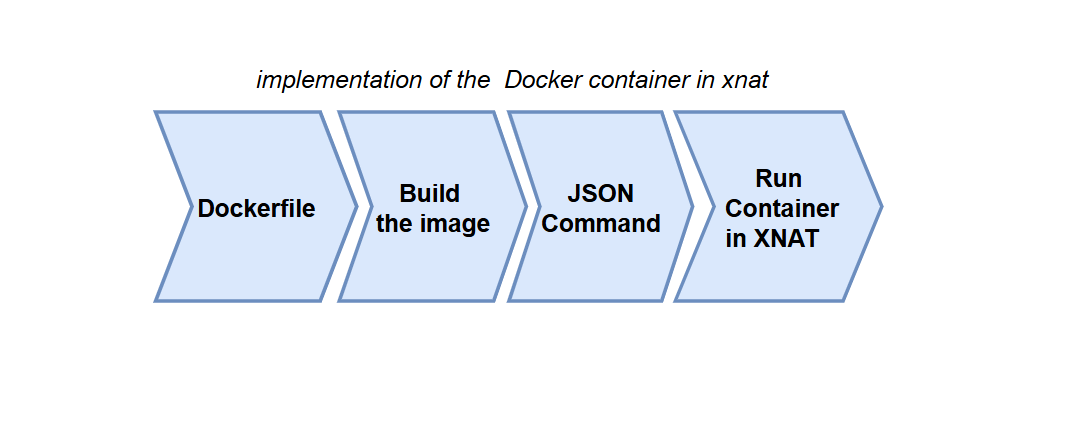
\includegraphics[width=0.9\linewidth]{en/content/ste.png}
    \caption{Diagram: the implementation of the docker Conatiner in xnat}
    \label{fig:enter-label}
\end{figure}






    

    \chapter{Implementation}

The purpose of this chapter is to introduce the system in more detail. A Python script is used to combine all the steps into an automated workflow. The libraries used in this work include: \texttt{requests}\footnote{\url{https://www.w3schools.com/python/module_requests.asp}accessed on 10 August 2025}, \texttt{json}\footnote{\url{https://www.w3schools.com/python/python_json.asp}accessed on 10 August 2025}, \texttt{os}\footnote{\url{https://docs.python.org/3/library/os.html}accessed on 10 August 2025}, \texttt{subprocess}\footnote{\url{https://docs.python.org/3/library/subprocess.html}accessed on 10 August 2025}, \texttt{getpass}\footnote{\url{https://docs.python.org/3/library/getpass.html}accessed on 10 August 2025}, \texttt{sys}\footnote{\url{https://docs.python.org/3/library/sys.html}accessed on 10 August 2025}, and \texttt{urllib3}\footnote{\url{https://urllib3.readthedocs.io/en/stable/}accessed on 10 August 2025}.

The use of the The Request library was for creating the interaction with the Web services of XNAT. The Python Requests library is the go-to solution for making HTTP requests in Python, thanks to its elegant and intuitive API that simplifies the process of interacting with web services and consuming data in the application.\footnote{\url{https://www.datacamp.com/tutorial/python-subprocess}accessed on 10 August 2025} The Sys module in Python provides access to variables and functions that interact closely with the Python interpreter and runtime environment. 

The fact that a JSON command is written, the use of the JSON library was necessary. JSON is a syntax for storing and exchanging data. it a text, written with JavaScript object notation.\footnote{schoolW3, Phython JSON}
The Python Subprocess module is a tool that allows to run other programs or commands from your Python code. Using the Python Subprocess module resembles executing commands directly on the system computer using Python instead of typing them directly into the command prompt. This module makes it easy to automate the Python code.\footnote{\url{https://www.datacamp.com/tutorial/python-subprocess}accessed on 10 August 2025}. Getpass() prompts the user for a password without echoing. The getpass module provides a secure way to handle the password prompts where programs interact with the users via the terminal.\footnote{\url{https://www.geeksforgeeks.org/python/getpass-and-getuser-in-python-password-without-echo/}accessed on 10 August 2025}
 The urllib3 was used to disable the InsecureRequestWarning, which is normally shown when requests connects to a site with an unverified SSL certificate. This approach helps keeping the output clean and free of unnecessary warnings during the run of the Script.
 Currently the System is running Docker Engine 28.3.0,The Docker Client version in use is 20.10.5+dfsg1, which communicates with the Docker Engine to issue commands and manage images and containers. The XNAT web application is running on version 1.9.1.1, as verified through the web interface. 
 

\begin{figure}
    \centering
    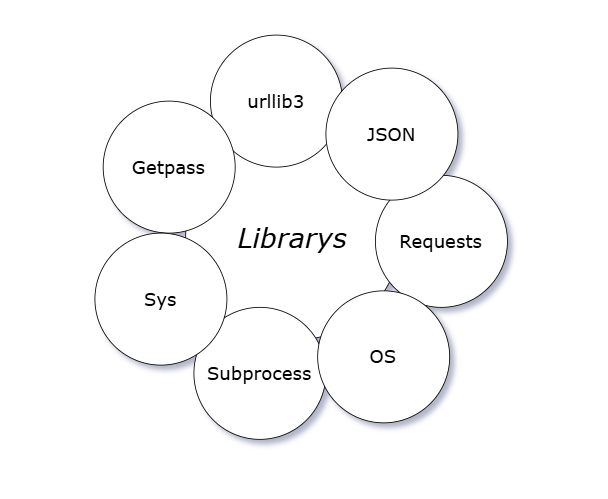
\includegraphics[width=0.7\linewidth]{en/content/lp.png}
    \caption{Schema: Core Libraries for Python Scripting in System Integration }
    \label{fig:enter-label}
\end{figure}


\section{Architecture and organization of the Code:}
 The automation script is structured into 17 distinct parts, each one is  responsible for a specific step in the overall workflow.
 During the development of the automation script, I closely followed the steps of the manual process, since I had already tested and completed it manually. which was writing a Container Script, writing a Dockerfile, building the image, writing a JSON Command and enabling the Command firstly on the Website and secondly on the Project, and the last step was completed by launching the Container. I carefully repeated the same steps during the implementation. In other words in every structured part is composed from a function that is responsible of doing a step of the manual Process.
 
 \section{The Dockerfile}
 
The first function is responsible for writing the Dockerfile is called \texttt{def write\_dockerfile} and it takes three arguments the target directory for the Dockerfile, the name of the Python script to include, and an optional base Docker image (defaulting to python:3.10-slim, currently the fastest and the slimmest image of docker). The function creates the necessary folder (if it doesn't already exist), constructs the Dockerfile content, and writes it. The content of the Dockerfile is introduced with a string interpolation and it contains the base image and numerous commands like WORKDIR /app (A working directory ) \texttt{COPY \{script\_filename\} /app/\{script\_filename\}} to copy the user script inside of the image. The line  RUN pip install \texttt{--no-cache-dir pandas} tells Docker to install the pandas Python library using pip during the build process of the Docker image.  which helps reduce the overall image size and avoids unnecessary layers in the building process. The last component of the Dockerfile is the \texttt{COPY requirements.txt /app/requirements.txt}, in this part it gives the opportunity for the user to write in a separate text file all the libraries used in the container script, which can be used later in the image build process.
The CMD instruction was removed from the Dockerfile because it caused errors when running the container in XNAT. The issue was due to a conflict between the CMD instruction in the Dockerfile and the Command. JSON configuration, as both included the python3 prefix. This led to a duplicate command execution, which caused the container to fail. By removing CMD in the Dockerfile, the execution logic is now fully controlled by XNAT through the JSON Command, ensuring a successful launch of the Container.

\begin{lstlisting}[language=bash,caption={Dockerfile}]
FROM python:3.10-slim
WORKDIR /app
COPY script.py /app/script.py
RUN pip install --no-cache-dir pandas
COPY requirements.txt /app/requirements.txt
\end{lstlisting}

The rest of the \texttt{def write\_dockerfile} ensures that the specified directory exists, then creates and writes a Dockerfile to that location. It constructs the full path to the file, writes the generated content into it, prints a confirmation message.


\lstset{
  language=Python,
  basicstyle=\ttfamily\small\color{black},
  keywordstyle=\color{black},
  identifierstyle=\color{black},
  stringstyle=\color{black},
  commentstyle=\color{black},
  numberstyle=\color{black},
  showstringspaces=false
}

\begin{lstlisting}
os.makedirs(docker_dir, exist_ok=True)
dockerfile_path = os.path.join(docker_dir, "Dockerfile")
with open(dockerfile_path, "w") as f:
    f.write(dockerfile_content)
print(f"Dockerfile written to {dockerfile_path}")
return dockerfile_path
\end{lstlisting}

This function ensures that the Dockerfile will be written in a appropriate way and it secures that all the dependencies are stored in the external requirement text file. It handles all possible cases and avoid the issues of errors and the Std in errors. 

\section{Building, Pushing and Tagging the image}

When a command is deployed in XNAT and a container is being launched, the first thing that XNAT is controlling if the docker image is available in the DockerHub. Which means the user has to have essentially a account in the Docker hub, and preferably to log himself before using the following script. consequently its essential to push and tag the image created.
The function responsible for the build is the \texttt{def build\_docker\_image}. and its expecting two parameters: 
\texttt{dockerfile\_path } for the Dockerfile path and the the name/tag for the Docker image to be built \texttt{docker\_image\_name}. For the build we used Subprocess.run to call the external docker build command.
usually when we want to build an image in docker we use the basic command \texttt{docker built  .} 


\begin{lstlisting}
 build_result = subprocess.run(["docker", "build", "-f", dockerfile_path, "-t", docker_image_name, "."],  capture_output=True, text=True)
    if build_result.returncode != 0:
        print(f"Build failed:\n{build_result.stderr}")
        sys.exit(1)
\end{lstlisting}

As we can see in this block it showing Subprocess.run was used  to call the external docker build command and the -f ,dockerfile\_path, tells Docker which Dockerfile to use.The  -t ,docker\_image\_name, sets the name and tag for the image. The point (.) at the end of the command means the current directory will be used as the build context. In addition the \texttt{capture\_output=True} collects both stdout and stderr so the script can handle their output or errors, and the text=True makes sure outputs are returned as strings.
\\Now that the image has been successfully built we can proceed to the next essential Step: "pushing the image to Docker Hub". In order to do that the same method by building of \texttt{subprocess.run} is used.


\begin{lstlisting}
full_tag = f"{dockerhub_username}/{docker_image_name}"
print(f"Pushing image to Docker Hub as '{full_tag}'...")
    push_result = subprocess.run(["docker", "push", full_tag], capture_output=True, text=True)
    if push_result.returncode != 0:
        print(f"Push failed:\n{push_result.stderr}")
        sys.exit(1)

\end{lstlisting}

In normal cases we use the command \texttt{docker push the image name}, and this assumes that the user is already logged in to their Docker account. However, in the automation script we make use of the \texttt{subprocess.run}. 
To explain this block,we begin by discussing the reason for using the full tag image. It constructs a full image tag in the Docker Hub format. Since the Docker Hub need image tags  to be in the format: The full image tag follows the format \texttt{dockerhub\_username/image\_name[:tag]}.

This line creates a correctly formatted name for your Docker image, so it links your Docker Hub account \texttt{(dockerhub\_username)} with the chosen image and optional version tag \texttt{(docker\_image\_name)}.

The line of the code: 
\begin{lstlisting}
push_result = subprocess.run(["docker", "push", full_tag], capture_output=True, text=True)
\end{lstlisting}
refers to the push process with the \texttt{subprocess.run} method. And it follows the same concept as builing the Docker image. 

\section{The Prompt Function for the required input:}

 This function performs the task of capturing input from the user.
 We have used this function in the script in multiple scenarios. First of them to take the Docker Hub user name from the user, in order to customize the JSON command we asked the user about the name of the Command and her description, And overall, it is used to take the username and password from the user's login credentials.The function proceeds through all of this steps by running the script.
 The function looks like this:
 
 \begin{lstlisting}
 def get_input(prompt):
    while True:
        value = input(prompt)
        if value.strip():
            return value
        else:
            print("Cannot be empty.")

\end{lstlisting}
The \texttt{ def get\_input} uses a while True loop to keep asking until the user enters a input, the \texttt{value.strip()} removes any whitespace from the user input.If the input is valid the value is returned, if it not the \texttt{Cannot be empty} will be printed.


\section{The JSON Command}

To communicate to XNAT the docker image, and consequently to run the container in the Web site. it is necessary to write a JSON Command. 
\footnote{https://wiki.xnat.org/container-service/json-command-definition}
Usually the JSON command is personalized and customized depending on the main idea of the image. But in the automation case the JSON command must be customized for all the cases, which means no matter which file is  selected still the command will handle it.
To achieve that the function used called \texttt{create\_json\_file},which builds the configuration dictionary for a Docker-based XNAT command (for the XNAT container service), writes it to a command.json file, and returns the filename.
The function expect three parameters:
\texttt{docker\_image} The Docker image to use (string),\texttt{script\_filename} The name of the Python script inside the container (string), \texttt{ mod\_data} :A dictionary holding user-provided metadata (names, descriptions, etc.)
Lets start analyzing the first block of the JSON command:
\begin{lstlisting}

json_file = {
        "name": mod_data["command_name"],
        "description": mod_data["command_description"],
        "version": "1.5",
        "type": "docker",
        "image": docker_image,
        "command-line": f"python3 /app/{script_filename} /input/#input_file# /output",
        "mounts": [
            {"name": "input", "path": "/input", "writable": False},
            {"name": "output", "path": "/output", "writable": True}
        ],
\end{lstlisting}


In this block we are  defining the name of the Command, add a description and specify the version and the type of the image.
The command line declares the actual command to run inside of the container when invoked by XNAT. The placeholder \# is a template substitution (not a Regex Expression)  that tells XNAT \texttt{ "When you launch the Docker command, replace \#input\_file\# with the actual file name/path that the user selected as input."}, it does not define what a valid file looks like. It marks a spot in the command where XNAT should "fill in" an actual value.

The mount configures the directory mappings (as Docker Volume) between XNAT and the Docker container. Most of the time two are used, the input and the output.
we specified the Path: "/input" in the container and if the container can write or just read the files  \texttt{Not writable or Writable}.

The second part of the JSON Command:


\begin{lstlisting}

 "inputs": [
            {
                "name": "input_files",
                "description": "Input files",
                "type": "files",
                "element_type": "file",
                "required": True,
                "mount": "input",
                "multiple": True
            }
        ],
        "outputs": [
            {
                "name": "result_file",
                "type": "file",
                "description": "Result file output",
                "mount": "output",
                "path": "."
            }
        ],
\end{lstlisting}


This block defines the parameters that a user must provide as a input file when launching the container. 
Let's break down each field:\\

the \texttt{The "name": "input\_files"}  This name is used in other parts of the JSON in references—such as placeholders in the command-line. In addition we add a optional human friendly description. The type means that the input accepts more than a file, not just text files or scans or numbers, and we specify that each element in the input is specifically a file with  the \texttt{"element"}.
The required \texttt{= true} is mainly to refer that if the input is not provided the command can not be run. The mount in this part links the input to a specific mount inside of the container. All files provided by the user will appear in the /input directory inside the container. With the \texttt{multiple : True} its indicated that the user can upload or select more than one file for this input.
The same logic applies for the output part the only point that needed to be referred to it more is the \texttt{"path": "."} and this means the output file will be in the top level of the \/output directory. and it allows more than one output file, use "type": "files" in the output block.

The final block in the Command JSON :

\begin{lstlisting}

 "xnat": [
            {
                "name": wrapper_name,
                "label": mod_data["label_name"],
                "description": mod_data["label_description"],
                "contexts": ["xnat:projectData"],  
                "external-inputs": [
                    { 
                        "name": "project",
                        "type": "Project",
                        "required": True,
                        "load-children": True
                    }
                ],
                "output-handlers": [
                    {
                        "name": "output",
                        "accepts-command-output": "result_file",
                        "as-a-child-of": "project",
                        "type": "Resource",
                        "label": "Results",
                    }
\end{lstlisting}

This block defines what will be displayed on the XNAT interface and it connects the docker command with XNAT's web interface and permission system. It controls how the command appears as a tool in XNAT, how it integrated with projects or other data and how input are handled.
The wrapper name is the technical name of the command inside XNAT, the \texttt{"label": mod\_data["label\_name"]} is a human-readable name shown in XNAT \ac{UI}. The \texttt{"description": mod\_data["label\_description"]} is a description for the tool/wrapper, shown when users browse tools in XNAT. For the context it referees where we want to appear the container in the interface of XNAT, since the main idea was to have one Container on top of the structure of XNAT, here \texttt{["xnat:projectData"]}means this command is available at the project level.
 In the external input external entities from XNAT are defined. The fact that we used Project as a context for the command, consequently we require in the external input a project to be selected, in more details the name and the type must be Project. This input must be provided that why \texttt{True} is written.
 We tell the XNAT with \texttt{"load-children": True:} to load (in the UI) the child objects of the project when showing this input.\\
 In the output-handlers part we control  how the outputs from your command are stored and shown in XNAT after job completion.\\
 This output-handler tells XNAT to take the result file the command produces, store it as a resource under the project, call that section “Results” in the UI. 
 The \texttt{as-a-child-of": "project"} reffers that the results are uploaded in XNAT project back as new resources.

 Finally the script writes the JSON Command file, ensuring that the JSON Command is saved in a correct format ready to be uploaded in XNAT.
 
 \section{Upload the Command in XNAT}

 After writing the JSON command the next step is to send it to XNAT, and to achieve this we have to use the appropriate REST API responsible for uploading the container Command in XNAT.
 We can find the list of all REST APIS under the \texttt{Administer->Site Administration->Miscellaneous->Development Utilities->Swagger} .
 To send the Command to XNAT we found that the responsible REST API for it is POST.\footnote{https://xnat-dev.gwdg.de/xapi/swagger-ui.html\#/command-rest-api}
 The function responsible for that is the \texttt{def send\_json\_to\_xnat} and it expecting four parameters: \texttt{json\_file\_path, xnat\_url, xnat\_user, xnat\_password}. Working with REST APIS we have to proceed at first with building the URL Endpoint for XNAT’s command registration.
 
\begin{lstlisting}
def send_json_to_xnat(json_file_path, xnat_url, xnat_user, xnat_password): 

    url = f"{xnat_url}/xapi/commands"
    print(f"Uploading command to {url}")
    with open(json_file_path, "r") as f:
        response = requests.post(url, auth=(xnat_user, xnat_password), json=json.load(f))
    if response.status_code == 200:
        print("Command uploaded successfully.")
    elif response.status_code == 201:
        print("Command created successfully.")
    elif response.status_code == 409:
        print("Command already exists.")
    else:
        print(f"Failed to upload command: {response.status_code} - {response.text}")

\end{lstlisting}

This function takes the path that describes the JSON Command, the base URL of the XNAT server, and the credentials for authentication. First it construct the correct REST API Endpoint by appending the /xapi/commands(xapi) to the provided XNAT URL, ensuring that the command is sent to the appropriate API for command registration. It then opens the JSON file, loads it contents, and sends this data as a POST request to the API endpoint using \ac{HTTP} Basic Authentication with the supplied username and password. After making the request the function examine the server's response and for every case the function provides a feedback, helping the user to quickly to understand if the command upload succeeded or if action is needed to resolve an issue. 

\section{Preparations to launch the Container}
The goal of the previous steps is to launch the container in XNAT, but before that we need to do some sort of preparations. Due to the automation principle we need to get some information out of the XNAT web site service, and in this case we use the REST APIS technic too.The first information that we need to extract after sending the JSON Command to XNAT is the \texttt{Command ID and the Wrapper ID}.
In order to do that. 
 
\begin{lstlisting}
def get_command_wrapper_id(xnat_host, xnat_user, xnat_password, command_name, wrapper_name=None):
 
    url = f"{xnat_host.rstrip('/')}/xapi/commands"
    try:
        resp = requests.get(url, auth=(xnat_user, xnat_password), verify=False)
    except Exception as e:
        print(f"Verbindungsfehler: {e}")
        sys.exit(1)
    if resp.status_code != 200:
        print(f"Fehler beim Abrufen der Commands: {resp.status_code}")
        sys.exit(1)
    data = resp.json()
    commands = data.get("commands", data) if isinstance(data, dict) else data

    for command in commands:
        if command.get("name") == command_name:
            if not wrapper_name:
                return command.get("id")
            
            for wrappers_field in ["xnat", "wrappers"]:
                for wrapper in command.get(wrappers_field, []):
                    if wrapper.get("name") == wrapper_name:
                        return wrapper.get("id") or wrapper_name
            print("no Wrapper found")
            sys.exit(1)
    print("Command nicht gefunden.")
    sys.exit(1)
\end{lstlisting}
The function takes as an input the the XNAT server’s hostname, user password, the name of the desired command,the name of a specific wrapper. It builds at first the correct XNAT REST API endpoint to list all the registered command on XNAT.
Upon receiving a response, the function checks for a successful status (200 OK) otherwise, it reports the failure and exits. If only a command ID is needed (no wrapper specified), it returns the command’s ID directly. If a wrapper name is provided, the function searches for the wrapper within possible sections of the command definition under XNAT or ‘wrappers’ fields—returning the wrapper’s ID upon match. If the specified command or wrapper cannot be found, the function clearly reports this to the user.
After receiving the Command ID and the Wrapper ID we proceed by enabling the command in the project and in the site wide. For that we use the two functions \texttt{def enable\_wrapper\_sitewide} and \texttt{ def enable\_wrapper\_for\_project}, which both of them expect parameters like server’s host name, user login and  password, and the extracted Command ID and the wrapper ID. It builds the desired XNAT REST API endpoint in this case we used the PUT REST API, it checks the status of the status of the process and gives to the user a feedback to track the code's status.

\section{The Extraction of all files from all Project structures}
The function used in this part is \texttt{def get\_all\_files\_all\_levels}, and it collects all the files in the Project data hierarchy (project, subjects, experiments/sessions, and scans) from an XNAT system using its REST API. We used the REST API Endpoint PUT for the extraction and it proceeds by authenticating with the XNAT server using the provided user credentials and starts by gathering project-level files, querying all resource folders at the project root and listing every file found within them.At every step, the function structures each file into a dictionary containing hierarchical information (such as the level—project, subject, experiment, scan—and the relevant IDs), the file name, the resource folder it was found in, and an absolute URI for straightforward retrieval. By the end, it returns a comprehensive list of all file records across all levels in the project. 

\begin{figure}
    \centering
    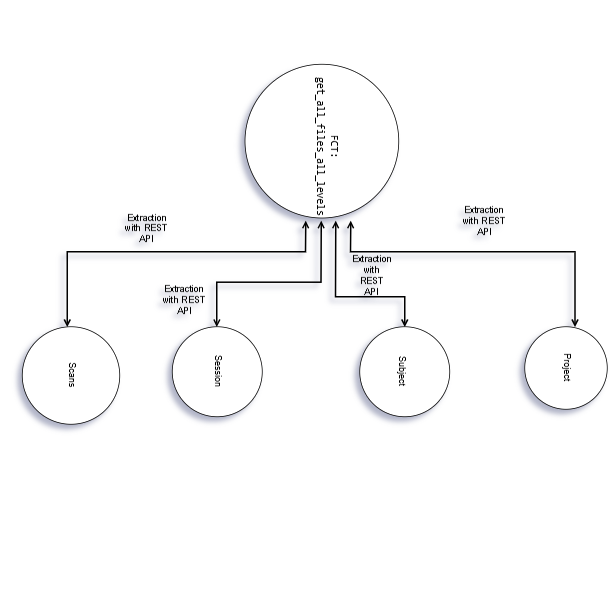
\includegraphics[width=0.9\linewidth]{en/content/edf1.png}
    \caption{Diagram: The Extraction of files from all the project structure}
    \label{fig:enter-label}
\end{figure}



\section{Launch the Container}
Arriving to the the famous part of launching the container we use the function \texttt{def launch\_container\_with\_all\_files}, this function is designed to automatically launch a container with all the files previously extracted as an input.It takes the XNAT server connection details, project and command identifiers, user authentication, the wrapper name, and a list of file to be processed. The function checks at the beginning if any file is provided. A payload dictionary is prepared, mapping the project ID and the input files string to the fields. The function next construct the appropriate URL for launching the command. Before sending the launch request, the function prints diagnostic information including the chosen files and payload, It submits a POST request with the payload as JSON and user credentials for authentication. After sending the request the Function report the user about the status and the responses.



\begin{lstlisting}
deflaunch_container_with_all_files(xnat_host,project_id,command_id,wrapper_name,xnat_user, xnat_password, files):
   
    if not files:
        print("no files found.")
        return 

    payload = {
        "project": project_id,
        "input_files": input_files_str
    }

    url = f"{xnat_host}/xapi/projects/{project_id}/commands/{command_id}/wrappers/{wrapper_name}/root/project/launch"

    headers = {"Content-Type": "application/json"}
    response = requests.post(
        url, auth=(xnat_user, xnat_password),
        headers=headers, json=payload, verify=False
    )

    print("Status:", response.status_code)
    print("Antwort:", response.text)
    if response.status_code in [200, 201, 202]:
        print("Container launched with all files!")
    else:
        print("failure :", response.status_code, response.text)
\end{lstlisting}

\begin{figure}
    \centering
    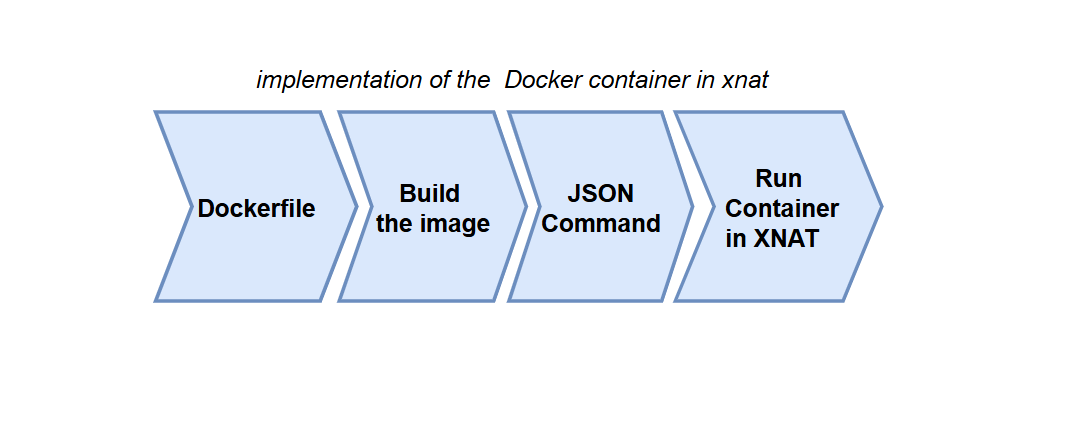
\includegraphics[width=0.9\linewidth]{en/content/Screenshot 2025-07-18 122044.png}
    \caption{Diagram: Implementation of Docker Container in XNAT}
    \label{fig:Implementation of Docker Container in XNAT}
\end{figure}





The Figure illustrates how the Automation script facilitate the process of deploying a Container in XNAt; It reduces all the steps. 


\begin{figure}
    \centering
    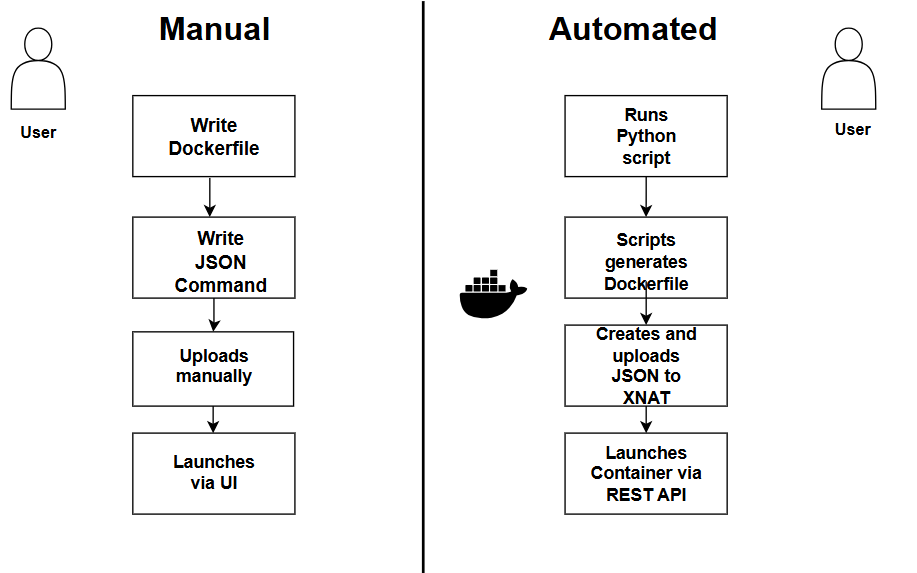
\includegraphics[width=0.6\linewidth]{en/content/o.png}
    \caption{Diagram illustrate the difference between the manual and the automatic process }
    \label{fig:enter-label}
\end{figure}

\begin{comment}
    https://wiki.xnat.org/documentation/strategies-for-xnat-image-data-storage
\end{comment}


\section{XNAT ML Plugin and The Pipeline}
For the purpose of Investigating and examining the Prototypical Implementation of
Automated Component Integrations in XNAT, it is relevant to cite the XNAT ML Plugin\footnote{ \url{https://wiki.xnat.org/ml/}accessed on 10 August 2025}. Which was previously a implementation method developed to incorporate machine learning workflows directly into XNAT. It offered capabilities for uploading, configuring, and training AI models. However, this approach was highly interdependent, the XNAT team officially deprecated the ML Plugin and the associated Datasets Plugin. They are no longer maintained or recommended for production use. An Other method that can be cited is the Pipeline Method.

Pipeline is a method of implementation for automated data processing in XNAT, using \ac{XML} descriptors and server-side scripts/tools. In XNAT, a pipeline is used to automate data processing workflows on imaging and related data stored in the
system. Pipelines allow researchers and developers to define and execute repeatable, structured sequences of
tasks such as data conversion, quality control, analysis, and post-processing directly on XNAT-managed data,without manual intervention.

After analyzing the Pipeline implementation method, it was revealed, that the architecture exhibits several limitations regarding scalability and flexibility, particularly when integrating new automated components.
The fact that these pipelines require direct access to the server via SSH in order to manually copy the XML
descriptor and associated scripts to a specific directory (/data/xnat/pipeline/pipelines/). This approach is not
feasible in secure or restricted settings where developers or researchers do not have shell access to the production
server. Furthermore, following the analysis of the REST API endpoint that XNAT supports, it became apparent that XNAT offers only limited support for this endpoint, the only endpoint that was supported in the list is \texttt{POST /pipelines/launch/{pipelineName}},This allows to programmatically launch an already registered pipeline in XNAT.  However, for full
automation, additional endpoints would be needed, such as one to enable a pipeline globally in XNAT and
another to assign or activate a pipeline for a specific project. These functionalities are currently not exposed via
the REST API, which means that while the execution of pipelines can be automated, the full deployment and
project-level configuration still require manual steps.
In conclusion, a fully automated pipeline workflow using only a Python script is not currently possible.
Only the launching of existing, pre-registered pipelines can be automated via REST.
  

    

    
\chapter{Testing and results}
\section{Testing the Code}
After testing the Code those are the results the we came to. 

 As we can see in the beginning  the process actively requests input from the user in order to proceed the implementation. it started by asking the user about his login credentials and then the Project ID that the user want to process, lastly before proceeding the creation and the command sending to XNAT, it asked the user about the command name and the description.
 After receiving  all the informations the script commence building the image, tagging, pushing, writing the JSON Command, enabling the Command, and lastly launch the container with all files.


 
 \section{Results on XNAT}
 The result that we came to after testing the code is that all the steps are working amazingly except that the container couldn't receive any files. with the \ac{STDout} view we found out that the Container received zero files. 
 
 \begin{figure}
    \centering
    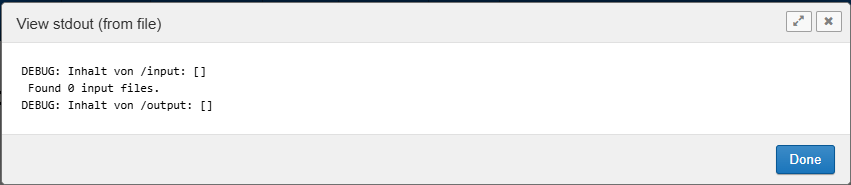
\includegraphics[width=0.9\textwidth]{en/content/STDOUT view.png}
    \caption{The STDout view of the Container on XNAT}
    \label{fig:enter-label}
\end{figure}

but weirdly after searching in the Container information, we noticed that the container in fact received the files and the file are listed in the input part of the container Input. 


\begin{figure}[p]
    \centering
    \rotatebox{90}{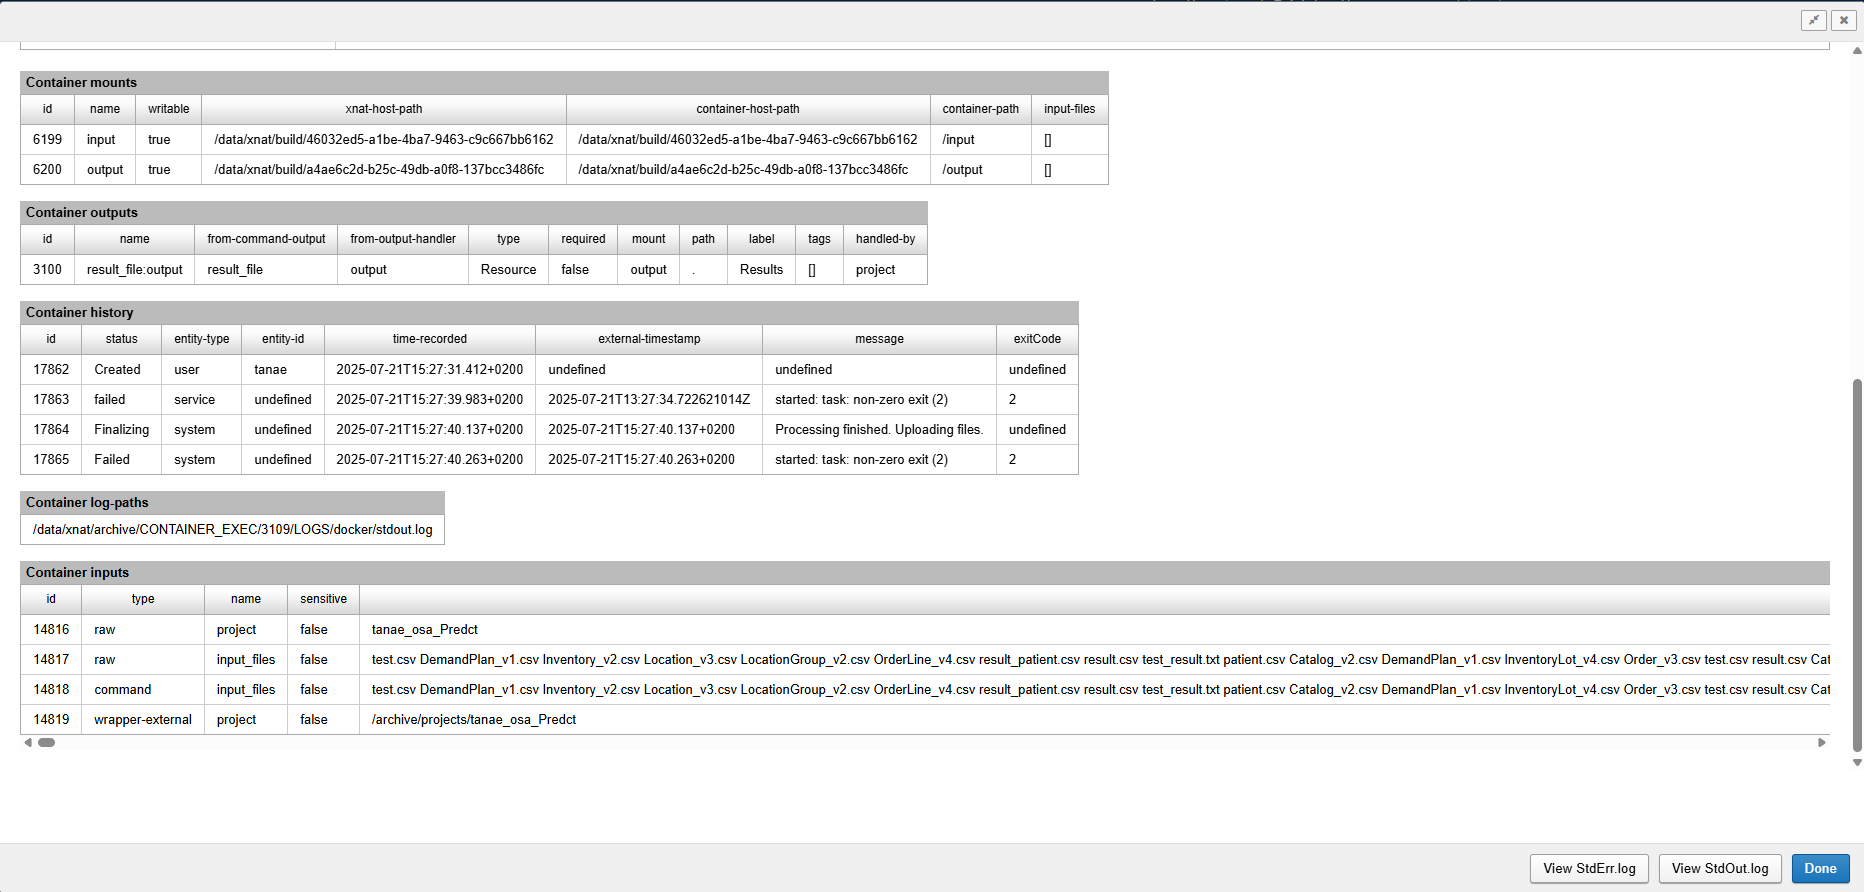
\includegraphics[width=0.95\textheight]{en/content/Container informatin 1.png}}
    \caption{Container Information 1}
    \label{fig:container-info-1}
\end{figure}


\begin{figure}
    \centering
    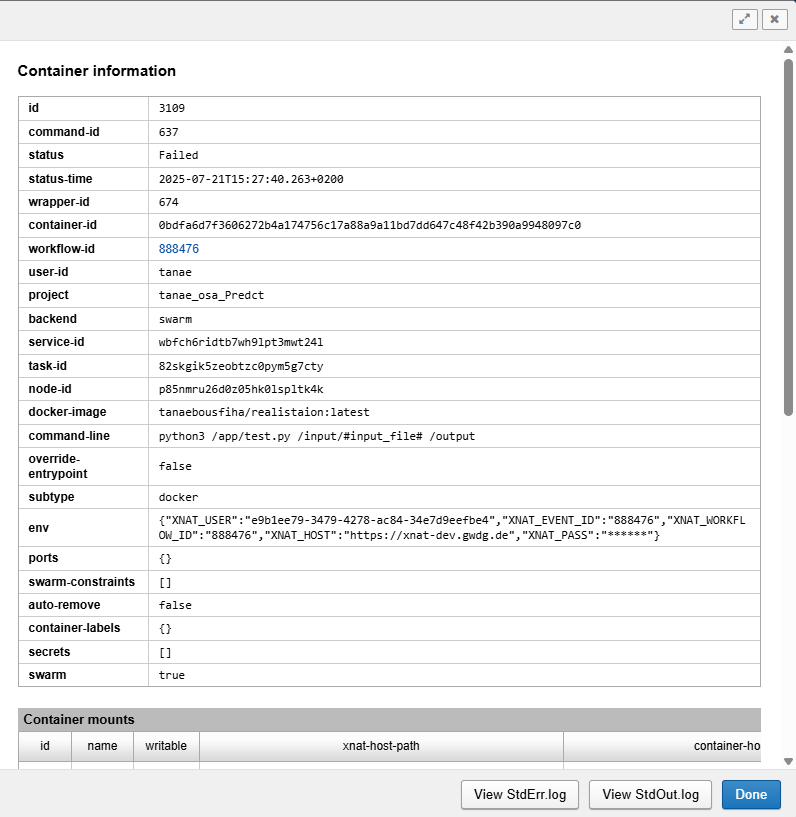
\includegraphics[width=0.9\linewidth]{en/content/Container information 2.png}
    \caption{Container Information 2 }
    \label{fig:enter-label}
\end{figure}

Details of the test procedure are described in Appendix A \cite{bousfiha2025appendix}..
.

The results demonstrate two things.  First, the automation script with the REST API worked correctly. Second, there is an issue with the container accessing the input files, despite them being listed as received.

    

    \chapter{Discussion}
In this chapter, the conclusion of ...

    



\chapter{Conclusion}


\section{Conclusion}
In this work, a framework was developed and automatized for executing machine learning models in the open-source medical Imaging and biosignals platform XNAT. This Paper presented the development and the Debugging process involved in integrating a Docker Container within the XNAT Environment for automated data processing.

Numerous Challenges made an appearance, first and foremost related to file input handling, container execution context, and the behavior of XNAT's data mounting system. Throughout repetitive testing and including diagnostic Scripting, REST API Integration, and JSON Command modifications, in spite of the fact that the core failures became comprehensible, a resolution to the underlying issue has not been achieved.


In Reply to These challenges, several countermeasures were proposed. These comprise implementing alternative procedures in Container scripts, ameliorating the Container logs for a better diagnostics. Furthermore, the analysis exposed deficiencies in XNAT’s temporary data handling and its limited error reporting capabilities, emphasizing the need for targeted improvements within the platform.

In a wider context, this work underline the complexity of the practice of integrating containers into clinical Research platforms.
Despite encountering technical constraints, the findings gained throughout the process
contribute valuable knowledge for future container based workflows in XNAT. The scripts and procedures developed form a pivotal step in establishing data processing pipelines that offer increased reliability and scalability. This work contributes meaningfully to the field of medical informatics, through this approach, it can be used in automated patient data processing, medical AI Workflow. It also provides a fast and efficient way to create new operations or updates, which can have positively a huge impact of the patient diagnosis or on the patient care in general.

The next phase involves a more in-depth examination of XNAT's mechanisms for handling file mounting at the system Level. Collaborating with XNAT developers or administrators may also help identify undocumented behaviors or system constraints. Additionally, exploring alternative methods for data Transfer such as Volume mounting from external storage or utilizing wrapper containers supporting the management of multiple files  might strengthen overall the results. Finally, transitioning from per-file execution to grouped workflows and container orchestration strategies could markedly increase scalability while minimizing processing demands in extensive project environments.


    

   %--- references ---
    \bibliographystyle{IEEEtran}
    \bibliography{content/references}
    \addcontentsline{toc}{chapter}{\bibname}
    \myemptypage
    
   %--- appendix ---
    \begin{appendix}
        
    

\appendix
\section{Test Protocol and Results}
\label{app:test}

\noindent\textbf{Author:} Tanae Bousfiha  
\noindent\textbf{Date:} August 2025  

\noindent This appendix documents the full terminal output of the automated Docker–XNAT integration script
\texttt{Projekt.py}.  
It includes the complete build, push, and wrapper activation process, as well as the execution log showing the files processed by the container.  
This section serves as a reproducibility record for the workflow described in Section~X.X of the main text.

\begin{lstlisting}
tanae@mi0082n:~/dockerfile/xnat-osa/Ziel2_osaAutomatisation$ python Projekt.py
XNAT Username: tanae
XNAT Password:
Project ID:  tanae_osa_Predct
Path to the Python script: test.py
Name des Commands: Realisation
Beschreibung des Commands: describes the Realistaion Process
Dockerfile written to ./Dockerfile
Docker Hub username (to push the image): tanaebousfiha
Building Docker image 'realistaion:latest'...
Image 'realistaion:latest' built successfully.
Tagging image as 'tanaebousfiha/realistaion:latest'...
Pushing image to Docker Hub as 'tanaebousfiha/realistaion:latest'...
Image successfully pushed: tanaebousfiha/realistaion:latest
Corrected command.json created.
Uploading command to https://xnat-dev.gwdg.de/xapi/commands
Command created successfully.
Command-ID: 637
Wrapper-ID: 674
Wrapper 'realistaion_wrapper' wurde global aktiviert.
Wrapper 'realistaion_wrapper' wurde im Projekt 'tanae_osa_Predct' aktiviert.
Start the Container.:
Dateien: ['test.csv', 'DemandPlan_v1.csv', 'Inventory_v2.csv', ... more than 700 files]
Container succesfully launched with all files!
\end{lstlisting}


        \myemptypage
    \end{appendix}




\end{document}

        



